\chapter{Gaokao Reform --- Equal Probability Admission}\label{app:gaokao}

The preceding appendix applied the framework to the fiscal substrate
of sovereign debt (\cref{app:govfi}).  This appendix applies it to
the \emph{human capital substrate}---the university admission system
that determines which agents enter the viability kernel of higher
education.  The central result is a \emph{disparity conservation law}:
total university capacity is conserved; only its distribution across
provinces is free.  The policy implication is that the current allocation
system is a \emph{sword}---a structural separator that assigns students
different viability probabilities based solely on their province of
registration---and that a population-proportional allocation
removes this sword entirely.

% ================================================================
\paragraph{Notation / 符号表.}
% ================================================================
The following symbols are used throughout this appendix.
\textcolor{water}{Blue} = structure/flow,
\textcolor{dao}{red} = disparity/inequality,
\textcolor{sword}{cyan} = reform/detection,
\textcolor{caution}{orange} = threshold warnings.

\begin{center}
\renewcommand{\arraystretch}{1.2}
\begin{tabular}{@{}lp{5.5cm}p{5.5cm}@{}}
\toprule
\textbf{Symbol} & \textbf{English} & \textbf{中文} \\
\midrule
\multicolumn{3}{@{}l}{\emph{Provincial state}} \\
$N_i$             & Exam takers in province $i$
                  & 第 $i$ 省报名人数 \\
$n$               & Number of provinces ($= 31$)
                  & 省份数 \\
$C$               & Total national 985 capacity
                  & 985 总招生容量 \\
$s_i$             & Slots allocated to province $i$
                  & 第 $i$ 省招生名额 \\
\midrule
\multicolumn{3}{@{}l}{\emph{Rates / 录取率}} \\
$R_i$             & Admission rate $= s_i / N_i$
                  & 录取率 \\
$\bar{R}$         & National avg $= C / \sum N_i$
                  & 全国平均录取率 \\
\midrule
\multicolumn{3}{@{}l}{\emph{Disparity / 不平等}} \\
$D$               & Disparity ratio $= \max R_i / \min R_i$
                  & 最大最小比 \\
$G$               & Gini coefficient of $\{R_i\}$
                  & 基尼系数 \\
$\sigma_R$        & Std.\ dev.\ of rates across provinces
                  & 录取率标准差 \\
\midrule
\multicolumn{3}{@{}l}{\emph{Reform models}} \\
$w_i$             & Province weight (equal: $w_i = 1$)
                  & 省份权重 \\
$\Delta$          & Score band width (points)
                  & 分数段宽度 \\
\bottomrule
\end{tabular}
\end{center}

% ================================================================
\section{The Current System / 现行制度}\label{sec:gaokao-current}
% ================================================================

China's national college entrance examination (高考) is taken by
approximately $N = \sum_{i=1}^{31} N_i \approx 12{,}350{,}000$
students annually (2024 data).  Each university allocates a
\emph{fixed quota} $s_i$ to each province, set by historical
precedent and political negotiation rather than by population
proportion.  The admission rate for province~$i$ is
\begin{equation}\label{eq:gaokao-rate}
  R_i = \frac{s_i}{N_i}.
\end{equation}

\begin{definition}[Disparity index / 不平等指数]\label{def:disparity}
The \emph{disparity ratio} is $D = \max_i R_i \;/\; \min_i R_i$.
The \emph{Gini coefficient} of the rate vector $\mathbf{R}
= (R_1, \ldots, R_n)$ is
\[
  G = \frac{1}{2n^2 \tilde{R}} \sum_{i,j} |R_i - R_j|,
  \qquad \tilde{R} = \frac{1}{n}\sum_i R_i.
\]
Perfect equality: $G = 0$, $D = 1$.
Maximum inequality: $G \to 1$, $D \to \infty$.
\end{definition}

\paragraph{2024 data / 2024年数据.}
Using publicly available data from Chinese education statistics
sources\footnote{%
  Sources: 中国教育在线 (eol.cn), 聚汇数据 (gotohui.com),
  知乎 (zhihu.com), 高考直通车 (gaokaozhitongche.com),
  网易 (163.com), 搜狐 (sohu.com).
  All figures are approximate; see \texttt{gaokao/data.py} for
  per-source annotations and confidence levels.},
the 2024 985-university admission rates are:

\begin{center}
\renewcommand{\arraystretch}{1.1}
\begin{tabular}{@{}llrr@{}}
\toprule
\textbf{Province / 省份} & & \textbf{Exam takers / 考生}
  & \textbf{985 rate / 录取率} \\
\midrule
\multicolumn{4}{@{}l}{\emph{Top 5 — highest rate / 录取率最高}} \\
天津 & Tianjin   &   70{,}800 & 5.81\% \\
北京 & Beijing   &   67{,}000 & 5.30\% \\
上海 & Shanghai  &   54{,}000 & 4.40\% \\
吉林 & Jilin     &  130{,}100 & 3.56\% \\
青海 & Qinghai   &   65{,}600 & 3.36\% \\
\midrule
\multicolumn{4}{@{}l}{\emph{Bottom 5 — lowest rate / 录取率最低}} \\
云南 & Yunnan    &  395{,}000 & 1.00\% \\
广东 & Guangdong &  768{,}000 & 0.98\% \\
贵州 & Guizhou   &  472{,}500 & 0.98\% \\
河北 & Hebei     &  928{,}000 & 0.96\% \\
河南 & Henan     & 1{,}360{,}000 & 0.84\% \\
\bottomrule
\end{tabular}
\end{center}

\begin{proposition}[2024 disparity / 2024年不平等]\label{prop:gaokao-disparity}
For 985-university admission rates across 31 provinces (2024):
\[
  D = 6.9\times, \qquad G = 0.310, \qquad
  \bar{R}_{\textup{weighted}} = 1.33\%.
\]
天津 (Tianjin, $N = 70{,}800$) has a 985 rate of $5.81\%$;
河南 (Henan, $N = 1{,}360{,}000$) has $0.84\%$.
河南 has $19\times$ more exam takers but $6.9\times$ worse
admission probability.
\end{proposition}

\begin{remark}[The sword is the quota / 刀就是名额]
\label{rem:gaokao-sword}
The admission quota $s_i$ is the sword.  It satisfies both conditions
from \cref{def:sword}: (1)~autonomous actuation---each university
sets its own quotas without external constraint; (2)~observability
failure---students in province $i$ cannot observe or influence the
quota-setting process.  The disparity $D = 6.9\times$ is not a
natural phenomenon; it is an artefact of the quota allocation,
which is neither population-proportional nor merit-based.
\end{remark}

% ================================================================
\section{Reform Models / 改革模型}\label{sec:gaokao-reform}
% ================================================================

We consider two alternative allocation rules, holding total
capacity $C = \sum_i s_i \approx 164{,}203$ fixed.

\begin{definition}[Equal-weight allocation / 等权分配]
\label{def:equal-weight}
Set $w_i = 1$ for all $i$.  Then
\[
  s_i^{\textup{eq}} = \frac{C}{n}
  \approx 5{,}297 \;\text{per province}.
\]
\end{definition}

\begin{definition}[Population-proportional allocation / 人口比例分配]
\label{def:pop-prop}
Set $w_i = N_i$.  Then
\[
  s_i^{\textup{pp}} = C \cdot \frac{N_i}{\sum_j N_j},
  \qquad
  R_i^{\textup{pp}} = \frac{s_i^{\textup{pp}}}{N_i}
  = \frac{C}{\sum_j N_j} = \bar{R}
  \;\;\text{(constant for all $i$)}.
\]
\end{definition}

\begin{proposition}[Reform comparison / 改革对比]
\label{prop:gaokao-reform}
Under the three allocation models:
\begin{center}
\renewcommand{\arraystretch}{1.1}
\begin{tabular}{@{}lrrr@{}}
\toprule
\textbf{Model / 模型} & \textbf{Gini ($G$)} & \textbf{$D$ (max/min)}
  & \textbf{Direction} \\
\midrule
Current / 现行制度  & $0.310$ & $6.9\times$ & --- \\
Equal-weight / 等权 & $0.514$ & $37.8\times$
  & \textcolor{dao}{$\uparrow$ worse} \\
Pop-proportional / 人口比例 & $0.0001$ & $1.0\times$
  & \textcolor{sword}{$\downarrow$ optimal} \\
\bottomrule
\end{tabular}
\end{center}
\end{proposition}

\begin{remark}[等权 $\neq$ 等概率 / Equal weight $\neq$ equal probability]
\label{rem:eq-neq-eqprob}
The na\"ive intuition that ``equal provincial weight'' produces
equality is \textbf{wrong}.  Equal absolute slots ($C/n$) distributed
to provinces of vastly different population sizes produces
\emph{worse} per-capita disparity: 西藏 ($N = 36{,}000$) would receive
a $14.7\%$ rate while 河南 ($N = 1{,}360{,}000$) would receive $0.39\%$.
The disparity ratio rises from $6.9\times$ to $37.8\times$.

The correct reform is population-proportional allocation:
$s_i \propto N_i$.  This gives every student the same probability
$R_i = \bar{R} \approx 1.33\%$ regardless of province.
\end{remark}

\begin{theorem}[Proportional allocation eliminates the sword]
\label{thm:gaokao-sword-removal}
Under population-proportional allocation $s_i = C \cdot N_i / N$
where $N = \sum_j N_j$:
\begin{enumerate}[label=\textup{(\alph*)}]
\item $R_i = C/N = \bar{R}$ for all $i$ (uniform rate);
\item $G = 0$ and $D = 1$ (perfect equality);
\item The quota $s_i$ ceases to be a sword: it no longer separates
  viability classes by province.
\end{enumerate}
\end{theorem}

\begin{proof}
(a) is immediate from the definition.  (b) follows since all rates are
equal.  For~(c), the sword conditions (\cref{def:sword}) fail:
the allocation is now a deterministic function of the publicly
observable population $N_i$, so observability holds and no autonomous
actuation remains.
\end{proof}

% ================================================================
\section{Within-Band Randomization / 分数段内随机化}
\label{sec:gaokao-band}
% ================================================================

The current system ranks students by exact score within each province.
A difference of one point (满分750, so $\Delta s = 1/750 \approx 0.13\%$
of the total range) can determine admission or rejection.  This creates
a ``one-point-one-fate'' (一分定终身) phenomenon.

\begin{definition}[Band randomization / 分数段随机化]
\label{def:band-random}
Fix a band width $\Delta > 0$ (e.g., $\Delta = 5$ points).
Partition the score range $[0, 750]$ into bands
$B_k = [k\Delta, (k+1)\Delta)$.
Within each band $B_k$, students are ranked by
\emph{uniform random permutation} rather than exact score.
\end{definition}

The effect: students whose scores differ by less than $\Delta$ have
equal probability of admission.  This converts a deterministic
(and fragile) ranking into a probabilistic one, eliminating the
incentive for one-point gaming while preserving the overall
meritocratic ordering at the $\Delta$-scale.

\begin{remark}[Band width choice / 分数段宽度选择]
\label{rem:band-width}
The choice $\Delta = 5$ is illustrative.  The optimal $\Delta$
balances two competing effects:
\begin{itemize}
\item Too small ($\Delta = 1$): equivalent to exact ranking,
  no randomization benefit.
\item Too large ($\Delta = 50$): too much noise, weakens
  the meritocratic signal.
\end{itemize}
The right $\Delta$ is an empirical question requiring the
fine-grained score distribution (一分一段表) to calibrate.
Score distributions for 2024 are publicly available for 29 of 31
provinces from provincial education examination authorities.
\end{remark}

% ================================================================
\section{Grace Period / 恩典期}\label{sec:gaokao-grace}
% ================================================================

The within-band randomization (\cref{sec:gaokao-band}) assigns each
student a \emph{tentative} school placement.  This initial assignment
is random within the score band.  The grace period converts this
random assignment into a \emph{chosen} one.

\begin{definition}[Grace period / 恩典期]\label{def:grace-period}
After the initial random-within-band assignment, a grace window
$[t_0, t_0 + \tau]$ opens during which students may \emph{swap}
placements with any other student in the same score band and the
same region, subject to the constraint that both students remain
within the same admission tier (budget).
\end{definition}

The mechanism has three phases:
\begin{enumerate}[label=\textup{(\alph*)}]
\item \textbf{Random seed / 随机初始.}
  Within-band randomization produces an initial assignment.
  No student chose this placement; it is the system's first offer.
\item \textbf{Grace window / 恩典窗口.}
  Students examine their assignment and may swap with willing
  partners in the same band and region.  You keep your tier
  but choose your specific school.  This is the time for the
  考生 to think: where do I actually want to go?
\item \textbf{Lock / 锁定.}
  After $\tau$, assignments become final.  No further swaps.
\end{enumerate}

\begin{remark}[Grace as bounded dissipation / 恩典即有界耗散]
\label{rem:gaokao-grace}
This is the same structure as the GovFi grace margins
(\cref{app:govfi}): bounded freedom within thresholds.
In GovFi, each layer $i$ has a grace margin $\epsilon_i = k_i - r$
within which losses are tolerated as legitimate costs.
In Gaokao, each student has a grace margin: freedom to swap
within the same tier without affecting the system's aggregate
allocation.

The grace period restores agency without restoring the sword.
The initial randomization removes one-point-one-fate (一分定终身);
the grace period gives back the student's choice of \emph{where},
while the population-proportional allocation determines \emph{how many}.
The constraint is the tier, not the specific school.

What is consumed during the grace period---the dissipated---is
information: students learn about their options, negotiate swaps,
discover preferences.  This is bounded dissipation in information
space, exactly analogous to the fiscal grace in \cref{app:govfi}.
\end{remark}

% ================================================================
\section{The Mean-Field Connection / 平均场联系}
\label{sec:gaokao-meanfield}
% ================================================================

The Gaokao disparity is a mean-field phenomenon in the sense of
\cref{sec:meanfield}.

\begin{proposition}[Sword = quota, mean = population share]
\label{prop:gaokao-meanfield}
Let $\bar{R} = C/N$ be the population-weighted national average.
Then:
\begin{enumerate}[label=\textup{(\alph*)}]
\item $13$ provinces (containing $67\%$ of all exam takers)
  have $R_i < \bar{R}$.
\item $18$ provinces (containing $33\%$ of all exam takers)
  have $R_i \geq \bar{R}$.
\item The unweighted arithmetic mean
  $\tilde{R} = \frac{1}{n}\sum R_i = 1.94\%$ exceeds $\bar{R} = 1.33\%$,
  showing that \emph{the majority of provinces have above-average rates
  when measured per province, but the majority of students have
  below-average rates when measured per capita}.
\end{enumerate}
\end{proposition}

This is the sword-is-the-mean phenomenon: the average computed
per province (unweighted, $\tilde{R}$) differs from the average
computed per student (weighted, $\bar{R}$), and this discrepancy
is itself the sword.  Most provinces appear ``above average'' while
most students are below it.

\begin{remark}[Importance sampling / 重要性抽样]
\label{rem:importance-sampling}
Why do the two averages disagree?  Because the current system
assigns importance weights in two levels:
\begin{enumerate}[label=\textup{(\arabic*)}]
\item \textbf{Level 1: equally to each province.}
  Every province gets the same voice---Tibet (3.6 万考生)
  counts the same as Henan (136 万考生), a 38:1 population
  ratio compressed to 1:1.
\item \textbf{Level 2: equally to each student within that province.}
  Within each province, students share their province's voice
  equally.
\end{enumerate}
The result: a student in Tibet inherits $1/36{,}000$ of a
full provincial vote, while a student in Henan inherits
$1/1{,}360{,}000$ of the same-sized vote.  Tibet's student
is 38 times louder than Henan's.  The importance weights
are the seed you plant---and the current system plants
unequal seeds.

In statistics, the fix is called \textbf{importance sampling}
(重要性抽样): if your sampling distribution $q$ differs from
the true distribution $p$, you multiply each sample by a
\emph{correction weight} $w(x) = p(x)/q(x)$:
\[
  \mathbb{E}_p[f(x)]
  \;=\;
  \mathbb{E}_q\!\Bigl[f(x)\,\cdot\,\frac{p(x)}{q(x)}\Bigr].
\]
Here $p$ is the per-student distribution (province $i$ has weight
$N_i/N$), $q$ is the per-province distribution (each province has
weight $1/n$), and $f$ is the admission rate.  The importance
weight is:
\[
  w_i \;=\; \frac{p_i}{q_i}
  \;=\; \frac{N_i/N}{1/n}
  \;=\; \frac{n\,N_i}{N}.
\]
Large provinces get large weights (Henan: $w \approx 3.4$),
small provinces get small ones (Tibet: $w \approx 0.09$).
The weighted average $\bar{R} = \sum w_i R_i / \sum w_i = 1.33\%$
is the true per-student mean.  The unweighted average
$\tilde{R} = 1.94\%$ is the \emph{biased} estimate that
ignores population---it over-counts small privileged provinces
and under-counts large disadvantaged ones.

In plain language (大白话): the unweighted mean is biased because
it lets 3.6 万 people in Tibet speak as loudly as 136 万 in Henan.
Importance sampling says: if you insist on giving every province
one vote, at least \emph{weight} those votes by how many students
each province actually has.  Once you do, $\tilde{R}$ collapses
to $\bar{R}$, and the illusion that ``most provinces are above
average'' disappears.
\end{remark}

\begin{remark}[Renormalization / 重整化]
\label{rem:gaokao-rg}
The importance weight assignment is a
\textcolor{dao}{renormalization group (RG) flow} compressed
into a single exam paper.  The current system has two scales:
\begin{center}
\renewcommand{\arraystretch}{1.15}
\begin{tabular}{@{}lll@{}}
\toprule
Scale & \textcolor{dao}{Current (bare)} & \textcolor{sword}{Reform (fixed point)} \\
\midrule
\textbf{Province} (coarse) & weight $= 1/n$ each
  & weight $= N_i/N$ \\
\textbf{Student} (fine) & weight $= 1/(n N_i)$
  & weight $= 1/N$ \\
\bottomrule
\end{tabular}
\end{center}
Under the \textcolor{dao}{current system}, the per-student
weight \emph{runs} with the province size $N_i$: a Tibet student
carries weight $1/(31 \times 36{,}000)$ while a Henan student
carries $1/(31 \times 1{,}360{,}000)$---a factor of 38.
The ``coupling constant'' (per-student admission probability)
\textcolor{dao}{depends on the scale at which you observe it}.
This is the signature of a system away from its RG fixed point.

Under \textcolor{sword}{population-proportional allocation}, every
student carries weight $1/N$ regardless of province.
The coarse-grained answer (per province: $s_i/N_i = C/N$)
and the fine-grained answer (per student: $C/N$) \emph{agree}.
The coupling no longer runs.
\textcolor{sword}{This is the RG fixed point}:
the admission probability is \emph{scale-invariant}---it does
not matter whether you measure at the province level or the
student level.

The current system's \textcolor{dao}{sword} is precisely the
RG anomaly: the bare parameter (per-province allocation) and
the physical observable (per-student probability) disagree.
Population-proportional allocation eliminates the anomaly by
making the bare parameter equal to the physical observable
at every scale.
\end{remark}

\begin{remark}[Temporal linearity / 时间线性]
\label{rem:gaokao-temporal}
The Gaokao happens every June.  It is non-pausable (you cannot stop the
exam mid-administration) and non-reversible (scores, once published,
determine that year's admissions permanently).  Each cohort passes
through the system exactly once.  This is temporal linearity: the
sword operates in real, non-replayable time.

The viability kernel $K$ is the set of provinces where a student's
probability of admission is at least $\bar{R}$.  Under the current
system, 13 provinces (67\% of students) are outside $K$.  Under
population-proportional allocation, $K$ expands to all provinces.
\end{remark}

% ================================================================
\section{Numerical Results / 数值结果}\label{sec:gaokao-numerics}
% ================================================================

The analysis is implemented in \texttt{gaokao/} (Python, stdlib only)
and reproduces the numbers in this appendix exactly.

\paragraph{Usage.}
\begin{verbatim}
  python -m gaokao.simulate
\end{verbatim}

\paragraph{Key outputs.}
\begin{center}
\renewcommand{\arraystretch}{1.1}
\begin{tabular}{@{}lrrr@{}}
\toprule
& \textbf{Current} & \textbf{Equal-wt} & \textbf{Pop-prop} \\
\midrule
Gini coefficient        & 0.310  & 0.514  & 0.0001 \\
Disparity ratio ($D$)   & 6.9$\times$ & 37.8$\times$ & 1.0$\times$ \\
Max rate (province)     & 5.81\% (天津)  & 14.71\% (西藏)  & 1.33\% (all) \\
Min rate (province)     & 0.84\% (河南)  & 0.39\% (河南)   & 1.33\% (all) \\
\bottomrule
\end{tabular}
\end{center}

Under population-proportional allocation, the top five gainers
by rate increase are: 河南 ($+0.49\%$), 河北 ($+0.37\%$),
广东 ($+0.35\%$), 贵州 ($+0.35\%$), 云南 ($+0.33\%$)---all
large-population provinces currently disadvantaged.
The biggest losers are the small, currently privileged provinces:
天津 ($-4.48\%$), 北京 ($-3.97\%$), 上海 ($-3.07\%$).

\begin{remark}[Data limitations / 数据局限]
\label{rem:gaokao-data}
The 985 admission rates used here are compiled from secondary sources
(media reports, data aggregators) rather than primary government
statistical yearbooks.  Some figures---particularly for mid-tier
provinces---are estimates based on ranges reported across multiple
sources.  The qualitative conclusions (6--7$\times$ disparity,
population-proportional reform eliminates it) are robust to
reasonable variations in the data.
Fine-grained score distributions (一分一段表) are available for
29 provinces in image format from provincial education examination
authority websites.  Text-format extraction would enable
within-band randomization calibration.
\end{remark}

\begin{remark}[Conservation law / 守恒定律 --- Log gas leakage]
\label{rem:gaokao-conservation}
Let $s_i$ denote the number of 985~slots allocated to province~$i$
under any method, and $C$ the total national 985~capacity.
The \textbf{slot conservation law} is
\[
  \sum_{i=1}^{n} s_i \;=\; C.
\]
The code checks four properties at each run:
\begin{enumerate}
  \item \emph{Slot conservation}: $\sum s_i = C$ (no slots created or destroyed).
  \item \emph{Non-negativity}: $s_i \ge 0$ for all~$i$.
  \item \emph{Capacity bound}: $s_i \le N_i$ (no province gets more slots
        than exam takers).
  \item \emph{Rate bounds}: $0 \le s_i / N_i \le 1$ (admission rate
        in $[0,1]$).
\end{enumerate}
The ``leak'' is $\ell = \sum s_i - C$.  A non-zero leak would indicate
an allocation error: slots appearing from, or disappearing into,
nowhere.  Both the equal-weight and population-proportional methods
pass with $\ell = 0$ (verified by \texttt{python -m gaokao.simulate}).

\textcolor{sword}{%
This is the same structure as the fiscal flow conservation check
(\cref{rem:govfi-conservation}):
$\text{leak} = \sum\text{inflow} - \sum\text{outflow}$.
Students flow through provinces the way money flows through
fiscal layers---conservation holds in both.}
\end{remark}

\bigskip
\noindent
\fbox{\parbox{\dimexpr\textwidth-2\fboxsep-2\fboxrule}{%
\smallskip
\textit{Author's note / 作者自述.}

\smallskip
\noindent
I took the Gaokao in Beijing in 2019 and scored 636.
Before that, I was a ``体育特长生'' (athletic recruit)---B-tier,
men's football---preparing for Tsinghua.
\textcolor{dao}{I failed.}  Not just at Tsinghua: at every university I tried.
So I took the Gaokao.

我在2019年在北京市参加了高考,考了636分。
在那之前,我是一个准备凭借高水平运动队招生(B类:男子足球)
考取清华大学的体育特长生。\textcolor{dao}{但我失败了}——不止在清华,
在我尝试过的每一所大学都失败了。然后,我就开始准备高考了。

\smallskip
I enrolled at Beijing University of Posts and Telecommunications,
majoring in Internet of Things Engineering.
I always thought I didn't like that school.
But I cannot deny: \textcolor{water}{I learned more there than I ever expected.}

我在北京邮电大学学习了两年,专业是物联网工程。
虽然我一直觉得我不喜欢这个学校,
但不可否认的是,\textcolor{water}{我在这里学到了很多——比我想象的更多。}

\smallskip
Two years later I transferred to New York University,
where I enrolled in Mechanical Engineering.
I graduated with a B.S.\ in Mechanical Engineering
and minors in Robotics and Mathematics.
\textcolor{water}{I liked learning math at the Courant Institute}---I took ODE
and combinatorics there, and that was about it.
I never took a functional analysis course.

之后我转学到了纽约大学,进入了机械工程专业。
我以机械工程学士学位毕业,辅修了机器人学和数学。
\textcolor{water}{我喜欢在Courant数学研究所学数学}——在那里修了常微分方程和组合数学,
仅此而已。我从来没有上过泛函分析的课。

\smallskip
In my second semester at NYU, I took Professor Ludovic Righetti's
\textit{Robotics: Locomotion and Manipulation}.
The course was not quite what the title promised (货不对板),
but I learned a great deal---most importantly, a question:
\textcolor{sword}{how should you think about AI?}
After that course I joined his Machines in Motion lab,
where Armand Jordana mentored me.
\textcolor{water}{He taught me how you should actually do math---and,
more importantly, how you should approach research.}

在纽约大学的第二个学期,我修了Ludovic Righetti教授的
\textit{Robotics: Locomotion and Manipulation}。
虽然货不对板,但我真的学到了很多——
最重要的,是一个问题:\textcolor{sword}{你该怎么看待AI。}
之后我加入了他的Machines in Motion实验室,
Armand Jordana在那里指导了我。
\textcolor{water}{他教会了我你到底应该怎么做数学——更重要的是,
你到底应该以怎样的态度做科研。}

\smallskip
When I applied to PhD programs, I was \textcolor{dao}{``全聚德'd''
again---rejected everywhere}.  Before that, I thought
I could get into MIT.
But the nice thing was: my advisor asked me if I wanted
to join his lab, and I said---\textcolor{sword}{of course!  Because this
happened to be exactly what I wanted.}

我在博士申请中再次被\textcolor{dao}{「全聚德」}了。在那之前,我以为我能上MIT来着。
但好在:我的导师问我愿不愿意加入他的实验室,
我说——\textcolor{sword}{当然!因为这恰恰正是我想做的事情。}
\smallskip
}}

\clearpage

\noindent
\fbox{\parbox{\dimexpr\textwidth-2\fboxsep-2\fboxrule}{%
\noindent
My advisor is Brian Plancher.  I believe he is the best GPU
programmer in the world---during his PhD \textcolor{water}{he hand-wrote a rigid
body dynamics library for robotics on GPU, from scratch.}
I picked up small tricks from him that actually worked,
and then I realised: maybe they are not tricks?
\textcolor{sword}{Maybe there is actually some math about it.
Then hence, Q.E.D.}

我的导师叫Brian Plancher,我认为他就是这个世界上最会写GPU代码的人——
因为他在博士期间,\textcolor{water}{自己手写了一个GPU上的刚体动力学仿真库。}
我从他那里学到了一些真正管用的小trick,然后我发现:
也许它们不是trick?\textcolor{sword}{Maybe there is actually some math about it.
Then hence, Q.E.D.}

\smallskip
Now I am a PhD student at Dartmouth College.  I live in a small
town called Lebanon.  My girlfriend visits often, and I am
genuinely fond of my colleagues---I think they are \textcolor{water}{real
scientists}, though they probably would not say so themselves.
They would say: \textcolor{water}{I just want to put my screws in the right place,}
so that when you need to assemble a robot, there are actually
screws to use.

现在我在Dartmouth College读博士,住在一个叫Lebanon的小镇。
我的女友时常来看我,我很喜欢我的同事们——
\textcolor{water}{我觉得他们就是真正的科学家},虽然他们可能不这么想。
她们会说:\textcolor{water}{我只是想把我的螺丝放好,}
这样当你想组装一个机器人的时候,真的有螺丝用。

\smallskip
One thing I can tell you for sure: \textcolor{water}{hand-crafting a robot
is really, really hard.}  This I know.

有一件事我可以肯定地告诉你:\textcolor{water}{手工造一个机器人,真的很难。}
这一点,我知道。

\smallskip
About one year later, \textcolor{sword}{I wrote this thesis.}

\medskip
\centerline{\textcolor{sword}{\textit{So, you just never know.  That is temporal linearity.}}}
\centerline{\textcolor{sword}{所以说,你永远不知道。这就是时间线性。}}

\smallskip
\centerline{\textcolor{sword}{这就是穿墙术。}}
\centerline{\textcolor{sword}{\textit{Follow some light, and try to even get a point.}}}
\centerline{\textcolor{sword}{\textit{A point of mass is all you need.}}}
\smallskip
}}

\bigskip
\begin{center}
\textit{任凭李俞江南鹤,都要低头求我怜!}

\smallskip
{\small --- 玉娇龙,\textit{卧虎藏龙}(李安)}
\end{center}

% ── 江湖诗 (from 笑傲江湖之东方不败) ──
\bigskip
\begin{center}
\textcolor{dao}{天下风云出我辈,一入江湖岁月催。}\\[3pt]
\textcolor{sword}{皇图霸业谈笑中,不胜人生一场醉。}\\[3pt]
\textcolor{dao}{提剑跨骑挥鬼雨,白骨如山鸟惊飞。}\\[3pt]
\textcolor{water}{尘事如潮人如水,只叹江湖几人回。}

\smallskip
{\small --- 黄霑,\textit{笑傲江湖之东方不败}(徐克)}
\end{center}

% ── 古筝 (standard 21-string guzheng — top-down view) ──
% Archived: 东方不败 sketch → appendices/archive_dongfang_bubai.tex
% Colours: sword (青冥) for strings/bridges, warm wood for body
\bigskip
\begin{center}
\definecolor{wood}{RGB}{160,110,60}         % 桐木 — paulownia warm brown
\definecolor{wooddark}{RGB}{120,78,40}      % 深木 — darker grain
\begin{tikzpicture}[line cap=round, line join=round, scale=0.9]
  % ═══════════════════════════════════════════════
  % Body outline (扁长方形, arched top face)
  % Left = 筝尾 (凤尾, narrow), Right = 筝首 (wide)
  % Height extended (~1.8 total spread vs original ~1.1)
  % ═══════════════════════════════════════════════

  % Soundboard fill (warm wood)
  \fill[wood!18]
    (-6.5, 0.85) .. controls (-4, 1.15) and (-1, 1.28)
    .. (2, 1.25) .. controls (4, 1.18) and (5.5, 1.02) .. (6.5, 0.85)
    -- (6.5, -0.9)
    .. controls (5.5, -1.05) and (4, -1.2) .. (2, -1.25)
    .. controls (-1, -1.22) and (-4, -1.08) .. (-6.5, -0.85)
    -- cycle;

  % Top edge (player-facing — gentle arc)
  \draw[line width=0.8pt, wooddark]
    (-6.5, 0.85) .. controls (-4, 1.15) and (-1, 1.28)
    .. (2, 1.25) .. controls (4, 1.18) and (5.5, 1.02) .. (6.5, 0.85);

  % Bottom edge (back)
  \draw[line width=0.8pt, wooddark]
    (-6.5, -0.85) .. controls (-4, -1.08) and (-1, -1.22)
    .. (2, -1.25) .. controls (4, -1.2) and (5.5, -1.05) .. (6.5, -0.9);

  % Left end — 筝尾 / 凤尾 (narrow)
  \draw[line width=0.8pt, wooddark]
    (-6.5, 0.85) -- (-6.5, -0.85);

  % Right end — 筝首 (wider)
  \draw[line width=0.8pt, wooddark]
    (6.5, 0.85) -- (6.5, -0.9);

  % ═══════════════════════════════════════════════
  % Sound holes (two rosettes near the ends)
  % ═══════════════════════════════════════════════
  \draw[line width=0.35pt, wooddark!50] (-5.5, 0) circle (0.28);
  \draw[line width=0.2pt, wooddark!30] (-5.5, 0) circle (0.16);
  \draw[line width=0.35pt, wooddark!50] (5.6, 0) circle (0.28);
  \draw[line width=0.2pt, wooddark!30] (5.6, 0) circle (0.16);

  % ═══════════════════════════════════════════════
  % Wood grain lines (subtle, on soundboard)
  % ═══════════════════════════════════════════════
  \draw[line width=0.1pt, wood!30]
    (-4, 0.3) .. controls (-1, 0.35) and (2, 0.3) .. (4.5, 0.25);
  \draw[line width=0.1pt, wood!30]
    (-4, -0.2) .. controls (-1, -0.25) and (2, -0.28) .. (4.5, -0.3);
  \draw[line width=0.08pt, wood!22]
    (-3.5, 0.6) .. controls (0, 0.65) and (3, 0.6) .. (4.8, 0.55);
  \draw[line width=0.08pt, wood!22]
    (-3.5, -0.55) .. controls (0, -0.6) and (3, -0.62) .. (4.8, -0.58);
  \draw[line width=0.06pt, wood!15]
    (-4.2, 0.85) .. controls (-1, 0.92) and (2, 0.88) .. (4.8, 0.78);
  \draw[line width=0.06pt, wood!15]
    (-4.2, -0.78) .. controls (-1, -0.85) and (2, -0.88) .. (4.8, -0.82);

  % ═══════════════════════════════════════════════
  % 左岳山 (left bridge — S-shaped)
  % ═══════════════════════════════════════════════
  \draw[line width=0.9pt, wooddark!80]
    (-4.8, 0.72) .. controls (-4.74, 0.3) and (-4.86, -0.25) .. (-4.8, -0.72);

  % ═══════════════════════════════════════════════
  % 右岳山 (right bridge — straight)
  % ═══════════════════════════════════════════════
  \draw[line width=0.9pt, wooddark!80]
    (5.0, 0.72) -- (5.0, -0.78);

  % ═══════════════════════════════════════════════
  % 21 strings (一弦一音, D major pentatonic)
  % 青冥 colour, thickening from high (1弦) to low (21弦)
  % ═══════════════════════════════════════════════
  \foreach \i in {1,...,21} {
    \pgfmathsetmacro{\ypos}{0.65 - (\i-1)*0.065}
    \pgfmathsetmacro{\lw}{0.08 + \i*0.02}
    \pgfmathsetmacro{\opac}{25 + \i*2.2}
    \draw[line width=\lw pt, sword!\opac]
      (-4.8, \ypos) -- (5.0, \ypos);
  }

  % ═══════════════════════════════════════════════
  % 雁柱 → 燕子 (bridges flipped to V — swallow silhouettes)
  % Each bridge: body (V dip) + swept wings (Chinese ink style)
  % ═══════════════════════════════════════════════
  \foreach \i in {1,...,21} {
    \pgfmathsetmacro{\ypos}{0.65 - (\i-1)*0.065}
    % Bridge x-position: sweeps from right to left
    \pgfmathsetmacro{\bx}{2.8 - (\i-1)*0.27}
    % Swallow body — V shape (flipped: dip down, wings up)
    \draw[line width=0.45pt, sword!65]
      (\bx-0.08, \ypos+0.03) -- (\bx, \ypos-0.08) -- (\bx+0.08, \ypos+0.03);
    % Left wing (swept back — ink brush flick)
    \draw[line width=0.25pt, sword!45]
      (\bx-0.08, \ypos+0.03)
      .. controls (\bx-0.16, \ypos+0.06) .. (\bx-0.22, \ypos+0.04);
    % Right wing (swept back — ink brush flick)
    \draw[line width=0.25pt, sword!45]
      (\bx+0.08, \ypos+0.03)
      .. controls (\bx+0.16, \ypos+0.06) .. (\bx+0.22, \ypos+0.04);
    % Tail fork (tiny V below body — the swallow's forked tail)
    \draw[line width=0.15pt, sword!35]
      (\bx-0.025, \ypos-0.12) -- (\bx, \ypos-0.08) -- (\bx+0.025, \ypos-0.12);
  }

  % ═══════════════════════════════════════════════
  % 弦钉 (tuning pins — right side)
  % ═══════════════════════════════════════════════
  \foreach \i in {1,...,21} {
    \pgfmathsetmacro{\ypos}{0.65 - (\i-1)*0.065}
    \fill[wooddark!55] (5.8, \ypos) circle (0.035);
  }

  % 弦钉 (string pegs — left side)
  \foreach \i in {1,...,21} {
    \pgfmathsetmacro{\ypos}{0.65 - (\i-1)*0.065}
    \fill[wooddark!45] (-5.8, \ypos) circle (0.03);
  }

  % Side thickness indication (shadow)
  \draw[line width=0.35pt, wooddark!20]
    (-6.5, -0.85) .. controls (-4, -1.15) and (-1, -1.3)
    .. (2, -1.35) .. controls (4, -1.28) and (5.5, -1.12) .. (6.5, -0.98);

  % ── Label ──
  \node[font=\scriptsize, text=sword!60] at (0, -2.0) {古筝 $\cdot$ 二十一弦};

  % ═══════════════════════════════════════════════
  % 广陵散 · 开指  (神奇秘谱, 朱权, 1425)
  % 指法 = motion primitives, not postures
  % Each diagram: string cross-section + fingertip trajectory
  %   approach (ghost) → contact → follow-through (bold arrow)
  % The arrow IS the primitive.  The string displacement is the effect.
  % ═══════════════════════════════════════════════

  \node[font=\small, text=sword!70] at (0, -2.9) {广陵散 $\cdot$ 开指};
  \node[font=\tiny, text=black!30] at (0, -3.25)
    {右手指法 --- 《神奇秘谱》(朱权,1425)};

  % ── Key: cross-section view (side view of 3 strings) ──
  % Player at BOTTOM of guzheng diagram (东方不败 plays from below)
  % Bottom = player side (近身);  Top = away from player (远身)
  % 向内 (inward, toward player) = ↓ downward
  % 向外 (outward, away from player) = ↑ upward
  % Each cell: 3 string dots (cross-section) + trajectory arrow

  % ── Biomechanical angles (right hand, palm-down, cross-section) ──
  % Player at bottom.  Thumb = inner/left, fingers = outer/right.
  % 大指 (thumb):  ~40° from vertical, tilted LEFT  (inner side of hand)
  % 食指 (index):  ~45° from vertical, tilted RIGHT (next to thumb)
  % 中指 (middle): ~80° from vertical, nearly STRAIGHT DOWN (longest finger)
  % Each 向内/向外 pair shares approach angle, reverses direction.

  % 托 — 大指向外 (thumb pushes outward ↑, from lower-LEFT at ~40°)
  \begin{scope}[shift={(-5.2, -4.8)}]
    \fill[sword!30] (-0.22, 0) circle (0.045);
    \fill[sword!50] (0, 0) circle (0.055);
    \fill[sword!30] (0.22, 0) circle (0.045);
    % Thumb approaches from lower-left (inner side of hand)
    \draw[line width=0.15pt, black!15, dashed]
      (-0.35, -0.48) -- (-0.12, -0.1);
    \fill[sword!55] (-0.08, -0.04) circle (0.035);
    \draw[-{Stealth[length=2.5pt]}, line width=0.7pt, sword!75]
      (-0.08, -0.04) -- (0.18, 0.48);          % sweeps up-right at ~40°
    % String bends up-right
    \draw[line width=0.3pt, sword!35]
      (-0.28, 0) .. controls (-0.1, 0.16) and (0.14, 0.14) .. (0.28, 0);
  \end{scope}

  % 抹 — 食指向内 (index pulls inward ↓, from upper-RIGHT at ~45°)
  \begin{scope}[shift={(-3.1, -4.8)}]
    \fill[sword!30] (-0.22, 0) circle (0.045);
    \fill[sword!50] (0, 0) circle (0.055);
    \fill[sword!30] (0.22, 0) circle (0.045);
    % Index approaches from upper-right, pulls down-left
    \draw[line width=0.15pt, black!15, dashed]
      (0.28, 0.48) -- (0.1, 0.12);
    \fill[sword!55] (0.06, 0.06) circle (0.035);
    \draw[-{Stealth[length=2.5pt]}, line width=0.7pt, sword!75]
      (0.06, 0.06) -- (-0.2, -0.46);           % pulls down-left at ~45°
    % String bends down-left
    \draw[line width=0.3pt, sword!35]
      (-0.28, 0) .. controls (-0.14, -0.14) and (0.1, -0.16) .. (0.28, 0);
  \end{scope}

  % 勾 — 中指向内 (middle pulls inward ↓, nearly VERTICAL from above)
  \begin{scope}[shift={(-1.0, -4.8)}]
    \fill[sword!30] (-0.22, 0) circle (0.045);
    \fill[sword!50] (0, 0) circle (0.055);
    \fill[sword!30] (0.22, 0) circle (0.045);
    % Middle finger: longest, approaches almost straight down
    \draw[line width=0.15pt, black!15, dashed]
      (0.04, 0.52) -- (0.02, 0.14);
    \fill[sword!55] (0.02, 0.08) circle (0.035);
    \draw[-{Stealth[length=2.5pt]}, line width=0.7pt, sword!75]
      (0.02, 0.08) -- (-0.02, -0.48);          % nearly vertical ↓
    % String bends straight down
    \draw[line width=0.3pt, sword!35]
      (-0.28, 0) .. controls (-0.12, -0.16) and (0.12, -0.16) .. (0.28, 0);
  \end{scope}

  % 剔 — 中指向外 (middle pushes outward ↑, nearly VERTICAL from below)
  \begin{scope}[shift={(1.1, -4.8)}]
    \fill[sword!30] (-0.22, 0) circle (0.045);
    \fill[sword!50] (0, 0) circle (0.055);
    \fill[sword!30] (0.22, 0) circle (0.045);
    % Middle finger: nearly vertical upward
    \draw[line width=0.15pt, black!15, dashed]
      (-0.04, -0.52) -- (-0.02, -0.14);
    \fill[sword!55] (-0.02, -0.08) circle (0.035);
    \draw[-{Stealth[length=2.5pt]}, line width=0.7pt, sword!75]
      (-0.02, -0.08) -- (0.02, 0.48);          % nearly vertical ↑
    % String bends straight up
    \draw[line width=0.3pt, sword!35]
      (-0.28, 0) .. controls (-0.12, 0.16) and (0.12, 0.16) .. (0.28, 0);
  \end{scope}

  % 挑 — 食指向外 (index pushes outward ↑, from lower-RIGHT at ~45°)
  \begin{scope}[shift={(3.2, -4.8)}]
    \fill[sword!30] (-0.22, 0) circle (0.045);
    \fill[sword!50] (0, 0) circle (0.055);
    \fill[sword!30] (0.22, 0) circle (0.045);
    % Index approaches from lower-right, pushes up-left
    \draw[line width=0.15pt, black!15, dashed]
      (0.28, -0.48) -- (0.1, -0.12);
    \fill[sword!55] (0.06, -0.06) circle (0.035);
    \draw[-{Stealth[length=2.5pt]}, line width=0.7pt, sword!75]
      (0.06, -0.06) -- (-0.2, 0.46);           % pushes up-left at ~45°
    % String bends up-left
    \draw[line width=0.3pt, sword!35]
      (-0.28, 0) .. controls (-0.14, 0.14) and (0.1, 0.16) .. (0.28, 0);
  \end{scope}

  % 撮 — 大指托↑ + 中指勾↓ simultaneous (pinch on two strings)
  \begin{scope}[shift={(5.3, -4.8)}]
    \fill[sword!50] (-0.22, 0) circle (0.055);  % string (thumb target)
    \fill[sword!25] (0, 0) circle (0.04);
    \fill[sword!50] (0.22, 0) circle (0.055);   % string (middle target)
    % Thumb: from lower-left, sweeps up-right at ~40° on left string
    \draw[line width=0.15pt, black!15, dashed]
      (-0.42, -0.4) -- (-0.28, -0.1);
    \fill[sword!55] (-0.24, -0.04) circle (0.03);
    \draw[-{Stealth[length=2pt]}, line width=0.6pt, sword!70]
      (-0.24, -0.04) -- (-0.08, 0.36);
    % Middle: from above, nearly vertical ↓ on right string
    \draw[line width=0.15pt, black!15, dashed]
      (0.24, 0.42) -- (0.22, 0.12);
    \fill[sword!55] (0.22, 0.06) circle (0.03);
    \draw[-{Stealth[length=2pt]}, line width=0.6pt, sword!70]
      (0.22, 0.06) -- (0.2, -0.36);
    % Strings displace in opposite directions
    \draw[line width=0.25pt, sword!30]
      (-0.38, 0) .. controls (-0.28, 0.12) .. (-0.08, 0);
    \draw[line width=0.25pt, sword!30]
      (0.08, 0) .. controls (0.16, -0.12) .. (0.38, 0);
  \end{scope}

  % ── Technique labels ──
  \node[font=\scriptsize, text=sword!65] at (-5.2, -5.6) {托};
  \node[font=\tiny, text=black!35] at (-5.2, -5.83)
    {大指$\uparrow$外};
  \node[font=\scriptsize, text=sword!65] at (-3.1, -5.6) {抹};
  \node[font=\tiny, text=black!35] at (-3.1, -5.83)
    {食指$\downarrow$内};
  \node[font=\scriptsize, text=sword!65] at (-1.0, -5.6) {勾};
  \node[font=\tiny, text=black!35] at (-1.0, -5.83)
    {中指$\downarrow$内};
  \node[font=\scriptsize, text=sword!65] at (1.1, -5.6) {剔};
  \node[font=\tiny, text=black!35] at (1.1, -5.83)
    {中指$\uparrow$外};
  \node[font=\scriptsize, text=sword!65] at (3.2, -5.6) {挑};
  \node[font=\tiny, text=black!35] at (3.2, -5.83)
    {食指$\uparrow$外};
  \node[font=\scriptsize, text=sword!65] at (5.3, -5.6) {撮};
  \node[font=\tiny, text=black!35] at (5.3, -5.83)
    {大$\uparrow$中$\downarrow$};

  % ═══════════════════════════════════════════════
  % 六脈神劍 annotation (金庸《天龍八部》)
  % Same 6 finger primitives → 6 hand meridians → 6 formless swords
  % 有質無形: the sword's definition in fictional representation
  % ═══════════════════════════════════════════════

  \node[font=\tiny, text=black!28, text width=11cm, align=center]
    at (0, -6.7) {%
    六脈神劍(金庸《天龍八部》):同以六指為基,%
    手太陰肺經 $\to$ \textcolor{sword!60}{少商}(拇),%
    手陽明大腸經 $\to$ \textcolor{sword!60}{商陽}(食),%
    手厥陰心包經 $\to$ \textcolor{sword!60}{中衝}(中),%
    手少陽三焦經 $\to$ \textcolor{sword!60}{關衝}(無名),%
    手少陰心經 $\to$ \textcolor{sword!60}{少衝}(小),%
    手太陽小腸經 $\to$ \textcolor{sword!60}{少澤}(小)。};

  \node[font=\tiny, text=black!28, text width=11cm, align=center]
    at (0, -7.55) {%
    「並非真劍,乃是以一陽指之指力化作劍氣,%
    \textcolor{sword!55}{有質無形},可稱無形氣劍。」%
    --- 有質無形者,即本文之刀:非實物,乃相函數。%
    常人六僧各習一脈(分佈式),段譽以北冥神功二百年內力獨運六脈(統一式)%
    --- 即平均場閾值之上下。};

  \node[font=\tiny, text=black!28, text width=11cm, align=center]
    at (0, -8.25) {%
    白居易《琵琶行》:「輕攏慢撚\textcolor{sword!55}{抹}復\textcolor{sword!55}{挑}」%
    --- 同指法,異介質(氣/弦),同代數。};

  % ═══════════════════════════════════════════════
  % 绣花针 (embroidery needle — silver, with red thread)
  % 东方不败's weapon: the finest manipulation primitive
  % ═══════════════════════════════════════════════

  % Needle shaft (silver — long, thin, tapering)
  \draw[line width=0.6pt, black!25]
    (-2.2, -11.75) -- (2.5, -11.75);            % body
  \draw[line width=0.35pt, black!18]
    (2.5, -11.75) -- (3.2, -11.75);             % taper toward tip
  \draw[line width=0.12pt, black!35]
    (3.2, -11.75) -- (3.6, -11.75);             % tip (fine, sharp)
  % Tip point
  \fill[black!40] (3.6, -11.75) circle (0.015);
  % Needle eye (small oval at blunt end)
  \draw[line width=0.25pt, black!30]
    (-2.2, -11.75) ellipse (0.04 and 0.06);
  % Highlight (silver sheen — thin white line along shaft)
  \draw[line width=0.15pt, white]
    (-1.8, -11.72) -- (2.0, -11.72);

  % Red thread (trailing from eye — flowing, alive)
  \draw[line width=0.35pt, dao!65]
    (-2.24, -11.75)
    .. controls (-2.8, -11.55) and (-3.2, -11.85) .. (-3.6, -11.5)
    .. controls (-4.0, -11.15) and (-4.3, -11.6) .. (-4.6, -11.25)
    .. controls (-4.85, -10.95) and (-5.1, -11.3) .. (-5.3, -11.1);
  % Thread thins at the trailing end
  \draw[line width=0.2pt, dao!45]
    (-5.3, -11.1)
    .. controls (-5.5, -10.9) and (-5.7, -11.15) .. (-5.85, -11.0);
  \draw[line width=0.1pt, dao!28]
    (-5.85, -11.0)
    .. controls (-6.0, -10.85) and (-6.1, -11.05) .. (-6.2, -10.95);

\end{tikzpicture}
\end{center}

% ── 琵琶行 (白居易, 元和十一年 / 816 CE) ──
% Position: the user is the 琵琶女.
% water = music / river / flow / peak;
% dao = loss / exile / cutting / decline;
% sword = recognition / phase transition / detection

\bigskip
\begin{center}
{\small\bfseries 琵琶行}\\[2pt]
{\small 白居易}
\end{center}

\smallskip
\begin{center}
\parbox{0.85\textwidth}{\small\textcolor{black!45}{%
元和十年,予左迁九江郡司马。明年秋,送客湓浦口,闻舟中夜弹琵琶者,听其音,铮铮然有京都声。问其人,本长安倡女,尝学琵琶于穆、曹二善才,年长色衰,委身为贾人妇。遂命酒,使快弹数曲。曲罢悯然,自叙少小时欢乐事,今漂沦憔悴,转徙于江湖间。予出官二年,恬然自安,感斯人言,是夕始觉有迁谪意。因为长句,歌以赠之,凡六百一十六言,命曰《琵琶行》。}}
\end{center}

\medskip
\begin{center}
% I. 江头送客
\textcolor{water}{浔阳江头夜送客,枫叶荻花秋瑟瑟。}\\[3pt]
\textcolor{water}{主人下马客在船,举酒欲饮无管弦。}\\[3pt]
\textcolor{dao}{醉不成欢惨将别,别时茫茫江浸月。}\\[8pt]
% II. 闻声 · 演奏
\textcolor{water}{忽闻水上琵琶声,主人忘归客不发。}\\[3pt]
\textcolor{water}{寻声暗问弹者谁,琵琶声停欲语迟。}\\[3pt]
\textcolor{water}{移船相近邀相见,添酒回灯重开宴。}\\[3pt]
\textcolor{sword}{千呼万唤始出来,犹抱琵琶半遮面。}\\[3pt]
\textcolor{water}{转轴拨弦三两声,未成曲调先有情。}\\[3pt]
\textcolor{dao}{弦弦掩抑声声思,似诉平生不得志。}\\[3pt]
\textcolor{water}{低眉信手续续弹,说尽心中无限事。}\\[3pt]
\textcolor{sword}{轻拢慢捻抹复挑,初为《霓裳》后《六幺》。}\\[3pt]
\textcolor{water}{大弦嘈嘈如急雨,小弦切切如私语。}\\[3pt]
\textcolor{water}{嘈嘈切切错杂弹,大珠小珠落玉盘。}\\[3pt]
\textcolor{water}{间关莺语花底滑,幽咽泉流冰下难。}\\[3pt]
\textcolor{dao}{冰泉冷涩弦凝绝,凝绝不通声暂歇。}\\[3pt]
\textcolor{sword}{别有幽愁暗恨生,此时无声胜有声。}\\[3pt]
\textcolor{dao}{银瓶乍破水浆迸,铁骑突出刀枪鸣。}\\[3pt]
\textcolor{dao}{曲终收拨当心画,四弦一声如裂帛。}\\[3pt]
\textcolor{water}{东船西舫悄无言,唯见江心秋月白。}\\[8pt]
% III. 琵琶女自述
\textcolor{water}{沉吟放拨插弦中,整顿衣裳起敛容。}\\[3pt]
\textcolor{water}{自言本是京城女,家在虾蟆陵下住。}\\[3pt]
\textcolor{water}{十三学得琵琶成,名属教坊第一部。}\\[3pt]
\textcolor{water}{曲罢曾教善才服,妆成每被秋娘妒。}\\[3pt]
\textcolor{water}{五陵年少争缠头,一曲红绡不知数。}\\[3pt]
\textcolor{water}{钿头银篦击节碎,血色罗裙翻酒污。}\\[3pt]
\textcolor{dao}{今年欢笑复明年,秋月春风等闲度。}\\[3pt]
\textcolor{dao}{弟走从军阿姨死,暮去朝来颜色故。}\\[3pt]
\textcolor{dao}{门前冷落鞍马稀,老大嫁作商人妇。}\\[3pt]
\textcolor{dao}{商人重利轻别离,前月浮梁买茶去。}\\[3pt]
\textcolor{dao}{去来江口守空船,绕船月明江水寒。}\\[3pt]
\textcolor{dao}{夜深忽梦少年事,梦啼妆泪红阑干。}\\[8pt]
% IV. 白居易 + 共鸣
\textcolor{dao}{我闻琵琶已叹息,又闻此语重唧唧。}\\[3pt]
\textcolor{sword}{同是天涯沦落人,相逢何必曾相识!}\\[3pt]
\textcolor{dao}{我从去年辞帝京,谪居卧病浔阳城。}\\[3pt]
\textcolor{dao}{浔阳地僻无音乐,终岁不闻丝竹声。}\\[3pt]
\textcolor{dao}{住近湓江地低湿,黄芦苦竹绕宅生。}\\[3pt]
\textcolor{dao}{其间旦暮闻何物?杜鹃啼血猿哀鸣。}\\[3pt]
\textcolor{water}{春江花朝秋月夜,往往取酒还独倾。}\\[3pt]
\textcolor{dao}{岂无山歌与村笛,呕哑嘲哳难为听。}\\[3pt]
\textcolor{sword}{今夜闻君琵琶语,如听仙乐耳暂明。}\\[3pt]
\textcolor{sword}{莫辞更坐弹一曲,为君翻作《琵琶行》。}\\[8pt]
% V. 结
\textcolor{water}{感我此言良久立,却坐促弦弦转急。}\\[3pt]
\textcolor{dao}{凄凄不似向前声,满座重闻皆掩泣。}\\[3pt]
\textcolor{water}{座中泣下谁最多?江州司马青衫湿。}

\smallskip
{\small --- 白居易,元和十一年(816)}
\end{center}

\bigskip
\begin{center}
% ── 甲骨文「中」── oracle bone script: a banner-pole through a ring
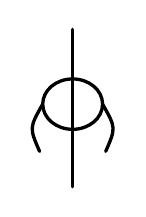
\begin{tikzpicture}[line width=1.2pt, line cap=round, line join=round]
  % Pole (vertical shaft)
  \draw (0,-0.9) -- (0,1.1);
  % Ring / target (slightly irregular, as in oracle bone style)
  \draw (0,0.15) ellipse (0.38 and 0.32);
  % Banner streamers (left and right, fluttering)
  \draw (-0.38,0.15) .. controls (-0.55,-0.15) .. (-0.42,-0.45);
  \draw ( 0.38,0.15) .. controls ( 0.55,-0.15) .. ( 0.42,-0.45);
\end{tikzpicture}

\smallskip
{\small\itshape zhǒng\,\raisebox{0.5ex}{\tiny$\checkmark$}}
\end{center}
